\documentclass[../main/main.tex]{subfiles}

\newdate{date}{7}{04}{2020}

\begin{document}

\marginpar{ \textbf{Lecture 9.} \\  \displaydate{date}. \\ Compiled:  \today.}


Now, considering that the system is homogeneous in space and in time (the hamiltonian is time independent), \( G^0 \) only depends on the difference between the spatial coordinates and times. Thus it is convenient to consider the Fourier transform of the Green's function:
\begin{equation*}
  G_{\alpha \beta }^0 (\va{x}t,\va{x}'t') = G_{\alpha \beta }^0 (\va{x}-\va{x}',t-t') \equiv
  \frac{1}{2 \pi V} \sum_{\va{k}}^{}
  \int_{- \infty }^{+ \infty } \dd[]{\omega } e^{i \va{k}\vdot (\va{x}-\va{x}')} e^{-i \omega (t-t')} G_{\alpha \beta }^0 (\va{k}, \omega )
\end{equation*}
Let us focus on the time-dependent of \( G^0_{\alpha \beta } \) and consider only  the first time dependent term of Eq.\eqref{eq:8_2}:
\begin{equation*}
  \Theta(t-t') e^{-i \omega (t-t') } \equiv \frac{1}{2 \pi } \int_{}^{} \dd[]{\omega } f(\omega )e^{-i \omega (t-t')}
\end{equation*}
where we have performed of course the Fourier transform with respect to the time variable.
The \( f(\omega ) \) can be obtained by a reverse integral over time of the left-hand side of the previous equation where we consider \( \tau \equiv t-t' \):
\begin{equation*}
\begin{split}
  f(\omega )&=  \int_{- \infty }^{+ \infty } \dd[]{\tau } e^{i \omega \tau } \qty[ \Theta (\tau ) e^{-i \omega _k \tau } ]
  = \int_{0}^{\infty } \dd[]{\tau }  e^{i(\omega -\omega _k)\tau }   =  \\
  &= \eval{\frac{e^{i(\omega - \omega _k) \tau } }{i( \omega - \omega _k)}}_0^\infty
  \overset{(a)}{=} \lim_{\eta  \rightarrow  0^+}
  \eval{\frac{e^{i(\omega - \omega _k + i \eta ) \tau } }{i( \omega - \omega _k + i \eta )}}_0^\infty = \\
  &= \lim_{\eta  \rightarrow  0^+} - \frac{1}{i} \frac{1}{(\omega - \omega _k + i \eta )} = \lim_{\eta  \rightarrow  0^+}  \frac{i}{(\omega - \omega _k + i \eta )}
\end{split}
\end{equation*}
where in step \( (a) \) in order  to make the integral convergent we have introduced a small positive quantity \( \eta >0 \).
Then, we repeat the same analysis for the second term of Eq.\eqref{eq:8_2}, obtaining a similar result:
\begin{equation*}
  \Theta(t'-t) e^{-i \omega (t'-t) } \longrightarrow  \lim_{\eta  \rightarrow  0^+} -  \frac{i}{(\omega - \omega _k - i \eta )}
\end{equation*}
By replacing the time dependent part with the Fourier expansion, one can rewrite the original non interacting Green's function as follow:
\begin{equation*}
\begin{split}
i G_{\alpha \beta }^0 (\va{x}t,\va{x}'t')  &= \frac{\delta _{\alpha \beta }}{2 \pi V} \sum_{\va{k}}^{} e^{i \va{k} \vdot (\va{x}-\va{x}')}
\Big[\Theta (\absvec{k} -k_f) \int_{- \infty }^{+ \infty } \dd[]{\omega } e^{- i \omega (t-t')} \frac{i}{\omega - \omega _k + i \eta } \\
& + \Theta (k_f-\absvec{k}) \int_{- \infty }^{+ \infty } \dd[]{\omega } e^{- i \omega (t-t')} \frac{i}{\omega - \omega _k - i \eta }  \Big]
\end{split}
\end{equation*}
and we notice that in the original Green's function (Eq.\eqref{eq:8_2}) we have a minus sign between the two terms, while in the Fourier transformed one there is a plus sign.
By using Eq.\eqref{eq:8_3}, we recover the explicit expression for the non-interacting Green's function in reciprocal space (in terms of the wave vector and of the frequency). Hence, we arrive at the expression of the Fourier transform of the non-interacting Green's funciton:
\begin{equation}
  G^0_{\alpha \beta } (\va{k}, \omega ) = \delta _{\alpha \beta } \qty[ \mathcolorbox{green!20}{\frac{\Theta (\absvec{k} - k_F )}{\omega - \omega _k + i \eta }}
  + \mathcolorbox{yellow!40}{\frac{\Theta ( k_F - \absvec{k} )}{\omega - \omega _k - i \eta }}]
  \label{eq:9_1}
\end{equation}
where the green term is valid for \( \va{k} \) vectors larger than the Fermi wave vector \( k_F \), which means for electrons that are created and destoryed outside the Fermi sphere. The second term is due to holes that are created or destroyed inside the Fermi sphere.

\begin{figure}[h!]
\centering
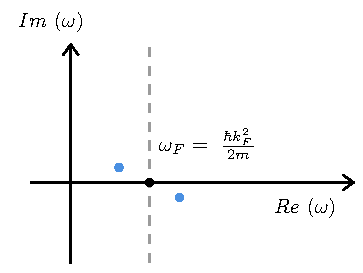
\includegraphics[width=0.6\textwidth]{../lessons/9_image/1.pdf}
\caption{\label{fig:9_1} Complex plane \( \omega  \), where \( \omega _F \) is the Fermi frequency.}
\end{figure}
Now, let us consider \( G^0_{\alpha \beta }  \) as a function in the complex \( \omega  \) plane in Fig.\ref{fig:9_1} (by also taking into account that of course the frequency is releated to energy with \( \omega _k = \varepsilon _k/ \hbar  = \hbar k^2 / (2m) \)).
\begin{itemize}
\item For a given \( \va{k} \) with \( \absvec{k}  >  k_F \)  there is a larger contribution whenever the denominator approaches zero. Exactly when the denominator is zero there is a single \textit{pole}  and the frequency is that is equal to \( \omega _p = \omega _k - i \eta  \) which is just below the real axis in Fig.\ref{fig:9_1}.

\item For a given \( \va{k} \) with \( \absvec{k}\le k_F  \) a single \emph{pole} is when \( \omega _p = \omega _k + i \eta  \)  which is just above the real axis in Fig.\ref{fig:9_1}.
\end{itemize}
This is an interesting result because we will see that something similar happen for a general interacting system Green's function.

To summarize, we have written explicitly the non-interacting Green's function both in the real space (Eq.\eqref{eq:8_2}) and reciprocal space (Eq.\eqref{eq:9_1}).
Using the Green's function we can compute the most interesting property of the system, as the ground state energy of the system \( E_0 \). We have already derived \( E_0 \) by using the second quantization approach, but it could be interesting to try to recover the ground state energy using the Green's function \( G_0 \).

\section{The Lehmann representation}
Now let us come back to the general Green's function by considering the case of \textbf{interacting} particles and let us try to show some other general properties of the Green's function. In particular, we are considering fermions but similar properties hold for bosons.

Let us rewrite the exact general Green's function as in Eq.\eqref{eq:7_1} (with \( \braket{\psi _0}{\psi _0} =1  \)):
\begin{equation*}
\begin{split}
i G_{\alpha \beta }(\va{x}t, \va{x}'t') \equiv & \bra{\psi _0} T \qty[ \hat{\psi }_{H \alpha } (\va{x},t) \hat{\psi }_{H_ \beta }^\dag (\va{x}',t')  ] \ket{\psi _0}  \\
= &\, \Theta (t-t') \bra{\psi _0}  \hat{\psi }_{H \alpha } (\va{x},t) \hat{\psi }_{H_ \beta }^\dag (\va{x}',t')  \ket{\psi _0} \\
& - \Theta (t'-t) \bra{\psi _0}  \hat{\psi }_{H_ \beta }^\dag (\va{x}',t')  \hat{\psi }_{H \alpha } (\va{x},t) \ket{\psi _0}
\end{split}
\label{eq:9_2}
\end{equation*}
where due to the effect of the time order operator, we have the sum of two contribution depending on the order of \( t \) with respect of \( t' \).
Let us focus only on the matrix element of the first term and we rewrite it by explicitly writing the Heisenberg field operators in terms of the ordinary field operators:
\begin{equation*}
  \bra{\psi _0}  \hat{\psi }_{H \alpha } (\va{x},t) \hat{\psi }_{H_ \beta }^\dag (\va{x}',t')  \ket{\psi _0}
  = \bra{\psi _0 }  e^{i \frac{\hat{H}t }{\hbar }} \hat{\psi }_ \alpha  (\va{x})
  e^{-i \frac{\hat{H}t }{\hbar }} e^{i \frac{\hat{H}t' }{\hbar }} \hat{\psi }_ \beta ^\dag (\va{x}') e^{-i \frac{\hat{H}t' }{\hbar }} \ket{\psi _0}
\end{equation*}
If we assume that \( \hat{H} \ket{\psi _0} = E_0 \ket{\psi _0}    \), we have already shown in the case of the demonstration that the Green function is uniform in time if the hamiltonian is time independent, that we can extract the exponential term from the matrix:
\begin{equation*}
    \bra{\psi _0}  \hat{\psi }_{H \alpha } (\va{x},t) \hat{\psi }_{H_ \beta }^\dag (\va{x}',t')  \ket{\psi _0}
    = e^{i \frac{E_0 (t-t')}{\hbar} }
    \bra{\psi _0 }  \hat{\psi }_ \alpha  (\va{x})
    e^{-i \frac{\hat{H} (t-t') }{\hbar }} \hat{\psi }_ \beta ^\dag (\va{x}')\ket{\psi _0}
\end{equation*}
Now let us consider the \emph{complete} set of all eigenstates of the system
\begin{equation*}
  \hat{H} \ket{\psi _n} = E_n \ket{\psi _n}, \qquad \sum_{n}^{} \ket{\psi _n} \bra{\psi _n} = \mathbb{1}
\end{equation*}
If we insert this complete set of states between the field operators we obtain:
\begin{small}
\begin{equation*}
\begin{split}
    \Theta (t-t') \bra{\psi _0}  \hat{\psi }_{H \alpha } (\va{x},t) \hat{\psi }_{H_ \beta }^\dag (\va{x}',t')  \ket{\psi _0} &=
    \sum_{n}^{}  e^{i \frac{E_0 (t-t')}{\hbar} }
    \bra{\psi _0 }  \hat{\psi }_ \alpha  (\va{x})
    e^{-i \frac{\hat{H} (t-t') }{\hbar }}  \ket{\psi _n} \bra{\psi _n} \hat{\psi }_ \beta ^\dag (\va{x}')\ket{\psi _0}  \\
    &= \sum_{n}^{}  e^{-i \frac{ (E_n-E_0) (t-t')}{\hbar} }
    \bra{\psi _0 }  \hat{\psi }_ \alpha  (\va{x})
  \ket{\psi _n} \bra{\psi _n} \hat{\psi }_ \beta ^\dag (\va{x}')\ket{\psi _0}
\end{split}
\end{equation*}
\end{small}
and similarly for the second term corresponding to \( \Theta (t'-t) \).
Hence, essentially the Lehman representation means using this trick.


Since the Green's function \( G \) is homogeneous in time (because the hamiltonian is time independent) it is convenient to take the \emph{partial} Fourier transform:
\begin{equation*}
  G_{\alpha \beta } (\va{x},\va{x}',t-t') = \frac{1}{2 \pi } \int_{- \infty }^{+ \infty } \dd[]{\omega } e^{- i \omega \tau } \widetilde{G}_{\alpha \beta } (\va{x},\va{x}', \omega )
\end{equation*}
with the Fourier transform instead of depending on two times, the Green's function depends only on one single frequency. In particular, it is a partial Fourier transform in the sense that it is the Fourier transform of the original Green's function only in terms of the time variable, while the space dependence remains the same.

One can compute this partial Fourier transform \( \widetilde{G}  \) by repeating a similar approach that we have used for the non-interacting Green's function. It is not necessary to repeat all the procedure, because actually we can exploit the similarity between this general case case and the previous non-interacting case.
Hence, in the Green's function in Eq.\eqref{eq:8_2} we have an exponential term related to time dependence and now for the general Green's function (Eq.\eqref{eq:9_2}) we have a similar term (of course by considering that the frequency is proportional to the energy):
\begin{equation*}
  \underbrace{e^{-i \omega _{\va{k}} (t-t')}}_{\text{in } G_0} = e^{-i \frac{\varepsilon _k (t-t')}{\hbar }}
  \longrightarrow  \underbrace{e^{-i \frac{(E_n-E_0)(t-t')}{\hbar }}  }_{ \text{in } G}
\end{equation*}
indeed we can again an exponential factor with the only difference that instead of \( \omega _k \) (or \( \varepsilon _k/\hbar  \)) we get this energy difference.
Thus, by using the same result obtained in the case of the non-interacting Green's function (Eq.\eqref{eq:9_1}) we obtain:
\begin{equation}
\begin{split}
\widetilde{G}_{\alpha \beta } (\va{x},\va{x}', \omega )   &=
\sum_{n}^{} \Big[ \frac{\bra{\psi _0} \hat{\psi }_ \alpha
 (\va{x}) \ket{\psi _n} \bra{\psi _n} \hat{\psi }_ \beta ^\dag (\va{x}') \ket{\psi _0}  }{\omega - \frac{(E_n-E_0)}{\hbar } + i \eta }
 +   \frac{\bra{\psi _0} \hat{\psi }_ \beta ^\dag (\va{x}') \ket{\psi _n} \bra{\psi _n}  \hat{\psi }_ \alpha
  (\va{x})  \ket{\psi _0}  }{\omega + \frac{(E_n-E_0)}{\hbar } - i \eta } \Big] \\
\end{split}
\label{eq:9_3}
\end{equation}
where we in particular note the presence of the poles.
As said, the denominators are just obtained by a similar approach as the corresponding denominators in the non-interacting Green's function. The frequency dependence is just trough those two denominators.

The last equation represent a \textbf{“meromorphic”} function, which is an analytic function over all the complex \( \omega  \) (frequency) plane, with the exception of a set of \emph{isolated} points (\textbf{poles}).
This is a generalization of the poles obtained in the non interacting case.
In particular, those poles (singularities) are of course found whenever the denominators are closed to zero and so we have poles when the frequency is given by this expression:
\begin{equation*}
  \omega = \pm \frac{(E_n-E_0)}{\hbar } \mp i \eta
\end{equation*}
This is a very interesting result because it generalizes what we have obtained in the case of the non-interacting Green's function.
The idea is that, as we will see in more details, while in the case of the non-interacting Green's function we had a single pole for a given \( \va{k} \) wave vector, in the case of the general full interacting Green's function we have a \emph{discrete} set of poles that are obtained by considering the situation when the denominators in Eq.\eqref{eq:9_3} vanishes.



Now, we try to understand better the meaning of the poles that we have seen looking at the denominator of this function.
First we recall the expression of the total number of particle operator in second quantization:
\begin{equation*}
  \hat{N} = \sum_{\alpha'}^{} \int_{}^{} \dd[]{\va{x}} \hat{\psi }_{\alpha'}^\dag (\va{x}) \hat{\psi }_{\alpha' } (\va{x})
\end{equation*}
Taking the commutator with the destruction field operator we obtain:
\begin{equation*}
  [\hat{N}, \hat{\psi }_{\alpha } (\va{x})] = - \hat{\psi }_{\alpha } (\va{x}) \quad \Rightarrow \hat{N} \hat{\psi }_{\alpha} (\va{x})  = \hat{\psi }_{\alpha } (\va{x}) (\hat{N}-1 )
\end{equation*}
Then, if we apply apply this sequnce of operators to the exact ground state of our system (which is a system made by \( N \) particles):
\begin{equation*}
  \hat{N}   \qty(  \hat{\psi }_{\alpha } (\va{x}) \ket{\psi _0} ) = (N-1) \qty(  \hat{\psi }_{\alpha } (\va{x}) \ket{\psi _0} )
\end{equation*}
This simply means that if \( \psi _0  \) is an eigenstate of the system with \( N \) particles, the application of the destruction field operator gives an eigenstate of \( \hat{N}  \) with eigenvalue\( (N-1) \).

Now consider that in the Lehmann representation we have introduced the complete basis set: \( \{ \ket{\psi _0}  \}   \) are eigenstates of the \emph{full} hamiltonian and in principle include \emph{all possible numbers} of particles.
Let us consider again the Eq.\eqref{eq:9_3} and in particular the first matrix element. The latter must be different from zero in order to not have a vanishing contribution when there is a pole:
\begin{equation*}
  \bra{\psi _0} \hat{\psi }_{\alpha } (\va{x}) \ket{\psi _n} \neq 0 \quad \text{ only if } M-1 = N  \Rightarrow M=N+1
\end{equation*}
where \( \ket{\psi _n} \) is an eigenstate of the system with \( M \) particles (where \( M \) is not necessarly equal to \( N \)), while \( \ket{\psi _0} \) is an eigenstate of the system with \( N \) particles. In the last formula we have obtained that in order to not have a vanishing contribution we must have states with the same number of particle both on the left and right; this is only possible if \( \ket{\psi _n}  \) is an eigenstate of the system with \( (N+1) \) particles.
The important conclusion is that in order to have a non vanishing matrix element, the eignestate \( \ket{\psi _n} \) must be an egeinstate of the system with one more particle! This is a peculiar effect different from the ordinary Schr$\ddot{o}$dinger equation where we must consider systems with the number of particles constant somehow.

Now, let us examine the corresponding denominator (of the latter matrix element) \( \omega - (E_n - E_0)/\hbar  + i \eta  \) and according to our observation, here the \( E_n \) energy is an eigenvalue of the system with \( (N+1) \) particles.
In the pole (singularity), hence whenever this denominator vanishes, we have the following situation:
\begin{equation}
\begin{split}
\omega   &= \frac{(E_n-E_0)}{\hbar }  - i \eta = \frac{E_n(N+1)}{\hbar } - \frac{E_0 (N)}{\hbar } - i \eta \\
&= \frac{1}{\hbar } \mathcolorbox{green!20}{\qty[ E_n (N+1) \mathcolorbox{yellow!40}{-E_0 (N+1)} ]} + \frac{1}{\hbar } \mathcolorbox{red!20}{\qty[ \mathcolorbox{yellow!40}{E_0 (N+1)} - E_0 (N)]} - i \eta
\end{split}
\label{eq:9_4}
\end{equation}
where we have added and substracted the same quantity \( E_0(N+1) \). The last expression is very interesting:
\begin{itemize}
\item if we look at the first term in green, clearly this is the difference between the energy corresponding to the \( n \) level and the energy corresponding to the ground state, for the system with \( (N+1) \) particles. In particular, this is the \textbf{excitation} energy of the system with \( (N+1) \) particles which can be written as:
\begin{equation*}
  \frac{1}{\hbar }\qty[ E_n (N+1) -E_0 (N+1) ] \equiv  \frac{\varepsilon _n (N+1)}{\hbar } \ge 0
\end{equation*}
indeed by definition of excitation energy is greater or equal than zero.

\item If we look at the second term in red, this is the difference between the ground states energy of the system with \( (N+1) \) and that with \( N \) particles. In physics this is a well known quantity called chemical potential\footnote{Read Chapter 2. of \cite{Fetter} for a review of this thermodynamic concept}.
The chemical potential is equivalent to the change in energy (at constant volume) of the ground states as one extra particle is added to the system. Thus we have:
\begin{equation*}
  \frac{1}{\hbar } \qty[ E_0 (N+1)- E_0 (N)] \equiv  \frac{\mu }{\hbar }
\end{equation*}

\end{itemize}
Eventually, in the pole:
\begin{equation}
  \omega = \frac{\varepsilon _n (N+1)}{\hbar } + \frac{\mu }{\hbar } - i \eta
  \label{eq:9_6}
\end{equation}
indeed in this pole the frequency is equal to the exictation energy plus the chemical potential and minus a small imaginary correction. The latter makes this pole frequency slightly below the real \( \omega  \) frequency axes.

Similarly considering the matrix element of the second term in Eq.\eqref{eq:9_3}, we can repeate the same procedure as above. Firstly, we check whenever this matrix element does not vanish:
\begin{equation*}
  \bra{\psi _0} \hat{\psi }_{\beta } ^\dag (\va{x}') \ket{\psi _n} \neq 0 \quad \text{ only if } M+1 =N \Rightarrow M = N-1
\end{equation*}
where again \( \ket{\psi _n} \) is an eigenstate of the system with \( M \) particles, while \( \ket{\psi _0} \) is an eigenstate of the system with \( N \).
In order to have a non vanishing contribution \( \ket{\psi _n}  \) must be an eigenstate of the system with \( (N-1) \) particles, hence with one less particle.
Then,  we can focus again on the corresponding denominator \( \omega + (E_n-E_0)/\hbar - i \eta  \) where \( E_n \) is an eigenvalue of the system with \( (N-1) \) particles.
In the pole:
\begin{equation}
\begin{split}
\omega   &= - \frac{(E_n - E_0)}{\hbar } + i \eta  =
- \frac{E_n (N-1)}{\hbar } + \frac{E_0 (N)}{\hbar } + i \eta  \\
&= - \frac{1}{\hbar } \mathcolorbox{green!20}{ \qty[E_n (N-1) \mathcolorbox{yellow!40}{- E_0 (N-1)}] }
+ \frac{1}{\hbar } \mathcolorbox{red!20}{ \qty[E_0 (N) \mathcolorbox{yellow!40}{- E_0 (N-1)}] } + i \eta
\end{split}
\label{eq:9_5}
\end{equation}
where again:
\begin{itemize}
\item the first green quantity is the \textbf{excitation} energy of the system with \( (N-1) \) particles and we can write
\begin{equation*}
  \frac{1}{\hbar } \qty[E_n (N-1) - E_0 (N-1)]  \equiv  \frac{\varepsilon _n (N-1)}{\hbar } \ge 0
\end{equation*}
\item the second red term is the difference between the ground states energy of the system with \( N \) and that with \( N-1 \) particles, which again is the chemical potential:
\begin{equation*}
  \frac{1}{\hbar }\qty[E_0 (N) - E_0 (N-1)] \equiv \frac{\mu }{\hbar }
\end{equation*}
\end{itemize}

\begin{remark}
In the chemical potential of Eq.\eqref{eq:9_4} we had the difference \( E_0(N+1)-E_0 (N) \), while in Eq.\eqref{eq:9_5} we had \( E_0(N)-E_0 (N-1)  \).
In the thermodynamic limit (\( N \rightarrow \infty  \)), the difference between the chemical potential of a system with \( N+1 \) particles and one with \( N \) is small because:
\begin{equation*}
  \mu (N+1) = \mu (N) + O \qty(\frac{1}{N})
\end{equation*}
\end{remark}

Eventually, in the pole:
\begin{equation}
  \omega = - \frac{\varepsilon _n (N-1)}{\hbar } + \frac{\mu }{\hbar } + i \eta
  \label{eq:9_7}
\end{equation}
where we have have minus the excitation energy of the system with \( N-1 \) particles plus the chemical potential and plus a small imaginary positive correction, which makes this frequency slightly above the real frequency  \( \omega  \) axes.


Finally, we can rewrite the Green's function in \eqref{eq:9_3} by explicitly reformulating the denominators using Eq.\eqref{eq:9_6} and Eq.\eqref{eq:9_7}:
\begin{equation}
\begin{split}
\widetilde{G}_{\alpha \beta } (\va{x},\va{x}', \omega )   &=
\sum_{n}^{} \Big[
\underbrace{
\frac{\bra{\psi _0} \hat{\psi }_ \alpha
 (\va{x}) \ket{\psi _n} \bra{\psi _n} \hat{\psi }_ \beta ^\dag (\va{x}') \ket{\psi _0}  }{\omega - \frac{\varepsilon _n (N+1)}{\hbar } - \frac{\mu }{\hbar } + i \eta }
 }_{I}
\underbrace{
+   \frac{\bra{\psi _0} \hat{\psi }_ \beta ^\dag (\va{x}') \ket{\psi _n} \bra{\psi _n}  \hat{\psi }_ \alpha
 (\va{x})  \ket{\psi _0}  }{  \omega + \frac{\varepsilon _n (N-1)}{\hbar } - \frac{\mu }{\hbar } - i \eta }
}_{II}
 \Big] \\
\end{split}
\label{eq:9_8}
\end{equation}
It is interesting to look at the behaviour of this function in the frequency plane (or in the \( \hbar \omega  \) frequency plane, so in the energy plane which is the same) as in Fig.\ref{fig:9_2}, where the poles are represented as crosses (the singularities are of course obtained letting the denominators of Eq.\eqref{eq:9_8} to go to zero). Note that there is a change of behaviour in correspondence of the chemical potential which distinguishes the part \( I \) of Eq.\eqref{eq:9_8} with the part \( II \). Clearly, we have that the poles are slightly above the real axes (red ones) if the energy is smaller than the chemical potential and slighly below the real axes (blue ones) if the energy is larger. This is a generalization for what we have found for non-interacting Green's function as in Fig.\ref{fig:9_1}. In this case we had only a single pole, just below or above the real axes, for given value of the \( \va{k} \) wave vector).


\begin{figure}[h!]
\centering
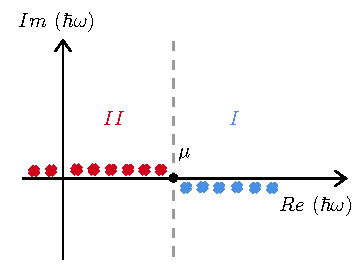
\includegraphics[width=0.6\textwidth]{../lessons/9_image/2.pdf}
\caption{\label{fig:9_2} Complex energy plane \( \hbar \omega  \). The blue crosses represent the poles of the part \( I  \) of Eq.\eqref{eq:9_8}, while the red crosses represent the poles of the part \( II \). We note that there is a change of behaviour in correspondence of the chemical potential.}
\end{figure}

In conclusion, we have found the dependence on the frequency of the general, exact Green's function! This ia a general Green's function, not an approximating one, appropiate for the interacting system.
To summarize, the poles go from above to below the real axis in the correspondence to the chemical potential of the system \( \mu  \).

The excitation energies of those excited states, for which the numerators do not vanish, are given by the singularities of the Green's function (Eq.\eqref{eq:9_8}). In particular they are:
\begin{itemize}
\item For the part \( I \):
\begin{equation}
  \varepsilon _n (N+1) = \hbar \Re (\omega _{pole}) - \mu
\end{equation}
\item For the part \( II \):
\begin{equation}
  \varepsilon _n (N-1) = -\hbar \Re (\omega _{pole}) + \mu
\end{equation}
\end{itemize}
Thus the Green's function gives information on the \textbf{excitation spectrum} of the system with \( N\pm1 \) particles.
Hence, we essentially have satisfied the promised property (anticipated in Sec.\ref{sec:7_1}) of the Green's function which states that it is able to describe the excitation spectrum of the system! Summarizing, to get the excitation energies of the system we can just consider the singularities (poles) of the Green's funciton.
To be more precise, of course we can get the excitation energies of those excited states for which the numerators do not vanish, otherwise it does not make any sense (if both the numerator and the denominator vanish at the same time, there are no more singularities).

The results obtained are of great importance to connect with experimental results. To ber more precise the Green's function can give informations on the excitation spectrum of the system with one more or one less particles.
Clearly, this is essentially a formal difference because we should still remember that in our case we are considering always the theromydynamic limit (\( N \rightarrow \infty  \)), so  \( N\pm 1 \) differ very little from \( N \).




















\end{document}
